%!TEX root = BSB.tex

\section{$\!\!\!\!\!\!\!$. Introduction and Background}    % Section 1

\subsection{Literature review}      % Section 1.1

Data defined on the finite discrete set $\bbN_{0:m} \teq \{0, 1, \dots, m\}$ widely exists in empirical research, and its essence is the counting observation constrained by the upper bound $m$. This kind of data is universal in biomedical fields (number of gene mutation sites detected), industrial engineering (number of product defects under fixed sampling) and social sciences (frequency statistics of discrete scoring options). The core value is to describe the mechanism of random events under the framework of limited resources. For instance, clinical trials need to evaluate the number of effective cases in a fixed sample size, and social surveys need to quantify the group tendency within the preset options. With the wide application of high-dimensional discrete data (such as gene expression matrix of single cell sequencing), the demand for theoretical deepening and model innovation of finite discrete distribution is increasingly prominent.

As the cornerstone of modeling finite discrete data, $\Binomial(m,p)$ distribution describes the probability distribution of the number of successful events $x$ in $m$ independent Bernoulli trials, whose \textit{probability mass function} (pmf) is
$$
   \Binomial(x|m,p) = \binom{m}{x} p^x (1-p)^{m-x}, \quad x \in \bbN_{0:m}.
$$
The core assumption of the model is the test independence and constant success probability $p$, which makes it a standard tool in quality control, medical statistics and other fields. However, the actual data often violate their ideal assumptions: first, the phenomenon of over-dispersion (the observation variance is significantly greater than $mp(1-p)$) is widespread in the actual data. Secondly, the homogeneous $p$ hypothesis is difficult to adapt to heterogeneous groups. Some traditional improvement methods, such as quasi-binomial model, which adjust variance by introducing dispersion parameters $\phi$, but fail to solve the essential defects of probability structure. And the generalized linear model (such as logistic regression) can introduce covariates to adjust $p$, its ability to deal with the unobserved heterogeneity is limited.

In order to address the issue that binomial distribution cannot fit finite discrete data with over--dispersion, scholars propose a  \textit{beta--binomial} (Beta-Bino) distribution from the Bayesian viewpoint, where the success probability $p$ is treated as a \trv and a $\mBeta(\al, \be)$ distribution is assigned as a prior of $p$, resulting in the pmf of $X \sim \BetaBino(m, \al, \be)$ as
\begin{eqnarray} \label{zyffour1.add1}
   \BetaBino(x|m, \al, \be) = \binom{m}{x} \frac{B(\al+x, \be + m-x)} {B(\al,\be)}, \quad x \in \bbN_{0:m},
\end{eqnarray}
where $B(a,b)$ represents the beta function. This improvement significantly improves the robustness of the model by quantifying the prior uncertainty. The super parameters $\al$ and $\be$ can be interpreted as ``the prior success/failure times", and their ratio $\al/(\al+\be)$ controls the prior mean, while $\al+\be$ adjusts the prior intensity. The variance
$$
   \frac{m\al\be(\al+\be+m)}{(\al+\be)^2(\al+\be+1)}
$$
of the model explicitly contains the over-dispersion correction term, and its superiority has been verified in the analysis of gene expression heterogeneity and social science survey data. However, it still has two major limitations: first, the subjectivity of the choice of super-parameters, the setting of $\al$ and $\be$ depends on prior knowledge, which results the inference under small samples are sensitive. Second is the lack of complex heterogeneity modeling, when the data has a hierarchical structure (such as different subgroups have different $p$ distribution), the standard model is difficult to capture population differences. Current research focuses on hierarchical Bayesian expansion: on the one hand, it introduces super prior distribution (such as $\al$ and $\be$ follow gamma distribution) to automatically learn the degree of dispersion. On the other hand, construct regression structure
$$
   \logit(p_i) = \ibx_{(i)}^{\T}\bbe + \varepsilon_i, \quad i=1,\ldots,n
$$
to integrate covariates, and combine MCMC sampling to realize full Bayesian inference. These developments are promoting the application of beta--binomial model in frontier scenarios such as drug dose-response curve fitting and online user behavior prediction.

In fact, in the hierarchical model, the prior distribution of $p$ does not necessarily have to be selected as beta distribution, but because beta distribution and binomial distribution are conjugate, which makes beta--binomial distribution have explicit expression and easy to calculate. On the contrary, the prior of $p$ can be regarded as any continuous distribution defined on the interval $[0,1]$, such as simplex, logit-normal, PIG distribution and a series of distributions proposed by Xunjian Li in the article. The arbitrary choice of prior distribution makes the model fitting too subjective, and it is impossible to judge the true prior of the data in the actual model fitting. Therefore, in this paper, we use Bernstein polynomial and Weierstrass approximation theorem to propose a general accurate prior expression, which can include all the prior special cases mentioned above. We call such a general distribution as Bernstein--Binomial distribution.

The rest of the paper will be organized as follows. In Section 1.2, we will introduce Bernstein polynomial and Weierstrass approximation theorem. In Section 2, we define Bernstein--Binomial distribution for the first time and use MM algorithm, DA algorithm and other methods to conduct statistical inference. The quantile regression model of Bernstein--Binomial distribution will also be studied and in Section 2.4. Some numerical experiments are presented in Section 3, which can prove the reliability of our model and the accuracy of corresponding algorithms. In Section 4, we will apply this new model to real data analysis and compare it with some traditional models. The conclusion and discussion of the results are stated in Section 5. Finally, the technical details and derivation involved in the paper will be supplemented in the appendix.


\subsection{Bernstein polynomials and Weierstrass approximation \\ theorem}     % Section 1.2

Given a non-negative integer $K$, Bernstein polynomials of order $K$ is a set of $K+1$ polynomials $\{B_{k,K}(\tau)\col k =0, 1, \dots, K\}$, where the individual polynomial
\begin{eqnarray} \label{zyffour1.1}
   B_{k,K}(\tau) \teq  \binom{K}{k} \tau^k (1-\tau)^{K-k}
   = \frac{1}{K+1} \cdot \mBeta(\tau| k+1, K-k+1), \quad \tau \in [0,1],
\end{eqnarray}
is sometimes called as the $k$-th Bernstein basis function of order/degree $K$, here $\mBeta(\cdot|a,b)$ denotes the \textit{probability density function} (pdf) of the $\mBeta(a, b)$ distribution. %Key Properties of Bernstein polynomials include

Bernstein polynomials are particularly useful in approximation theory.
Given a continuous function $f(\tau)$ on the interval $[0,1]$, the $K$-order \textit{Bernstein polynomial approximation} (BPA) is defined as
\begin{eqnarray}  \label{zyffour1.2}
   B_K(\tau|f) &\teq & \sum_{k=0}^K f(k/K) \cdot B_{k,K}(\tau)
   \sr{(\ref{zyffour1.1})}  \sum_{k=0}^K  \frac{ f(k/K)}{K+1} \cdot \mBeta(\tau|k+1, K-k+1) \non \\ [2mm]
   &=& \sum_{k=0}^K w_k \cdot \mBeta(\tau|k+1, K-k+1),  \quad \tau \in [0,1],
\end{eqnarray}
where $w_k \teq f(k/K)/(K+1)$. The formula (\ref{zyffour1.2}) indicates that the $K$-order BPA can be expressed as a linear combination of $K+1$ beta densities.

\begin{theorem} \label{thm1} {\rm  \textsf{(Weierstrass approximation theorem)}.  For any continuous function $f(\tau)$ defined on $[0,1]$, the $K$-order BPA $B_K(\tau |f)$ uniformly converges to $f(\tau)$; that is,
$$
   \lim_{K\to \infty} \sup_{\tau\in[0,1]} |B_K(\tau|f) - f(\tau) | = 0. \eqno{\|}
$$
}\end{theorem}

Consider a continuous \trv $X^* \in [0,1]$, if its pdf $f^*(\cdot)$ is a continuous function defined on $[0,1]$, then Theorem \ref{thm1} indicates that $f^*(\cdot)$ can be uniformly approximated by
\begin{eqnarray}  \label{zyffour1.3}
   \Bernstein(\tau|K, \bla) \teq \sum_{k=0}^K \la_k \cdot \mBeta(\tau|k+1,K-k+1), \quad \tau \in [0, 1].
\end{eqnarray}
The formula (\ref{zyffour1.3}) defines the pdf of a so-called $\Bernstein(K, \bla)$ distribution, where $K$ is a known non-negative integer (or a predetermined constant), and  $\bla = (\la_0,\la_1,\ldots,\la_K)^{\T}$ is an unknown parameter vector of weights satisfying $\bla \in \bbT_{K+1}$, where
\begin{eqnarray}   \label{zyffour1.4}
   \bbT_n \teq \left\{\ibx=(x_1, \dots, x_n)^{\T}\col 0 \le x_i \le 1, \; i=1, \dots, n, \; \ibx^{\T}\1_n = 1 \right\}
\end{eqnarray}
is the $n$-dimensional {\it closed} hyperplane, and $\1_n$ is the $n$-vector with each element being 1. For convenience, we define the $n$-dimensional {\it open} hyperplane as
\begin{eqnarray}   \label{zyffour1.5}
   \bbT_n^{\rm open} \teq \left\{\ibx=(x_1, \dots, x_n)^{\T}\col 0 < x_i < 1, \; i=1, \dots, n, \; \ibx^{\T}\1_n = 1 \right\}.
\end{eqnarray}

Because the Bernstein basis functions $\{B_{k,K}(\tau) \col k = 0, 1, \ldots, K\}$ are linearly independent on the interval $[0,1]$ and forms the basis of a $(K+1)$-dimensional polynomial space. That is, any polynomial with a degree not exceeding $K$ can be uniquely represented as a linear combination of these basis functions. Therefore, the scaled beta distribution $\{\mBeta(\tau|k+1,K-k+1) \ | \ k = 0,1,\ldots,K\}$ is also linearly independent, ensuring the uniqueness and parameter identifiability of the Bernstein distribution as a finite discrete mixture of beta distributions.
\begin{figure}[H]
    \subfigure[$\;$ $\mbox{Logit-N}(-1,1)$]
    {
        \centering
        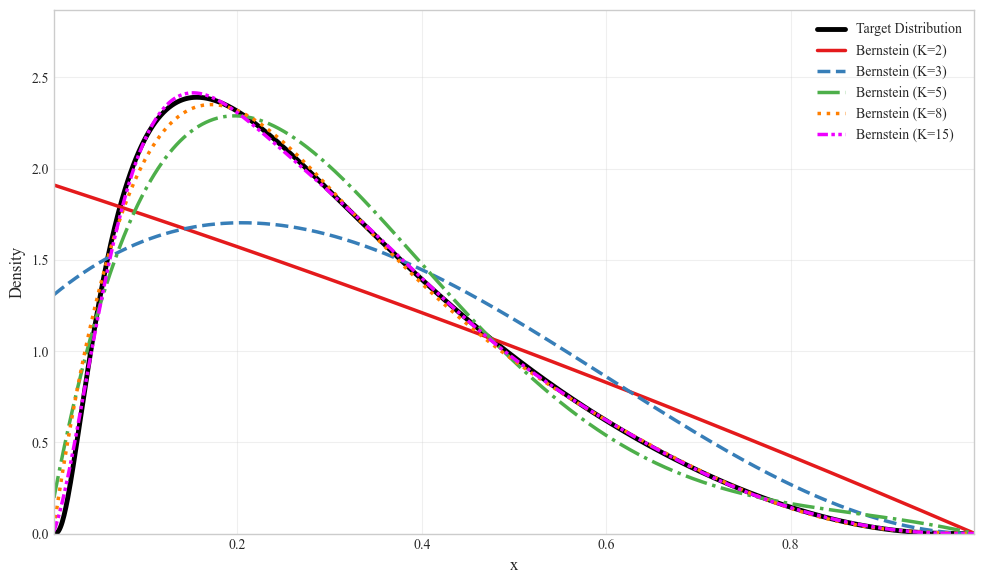
\includegraphics[width=0.5\linewidth]{figures/plot1.png}
    }
    \subfigure[$\;$ $\mBeta(2,5)$]
    {
        \centering
        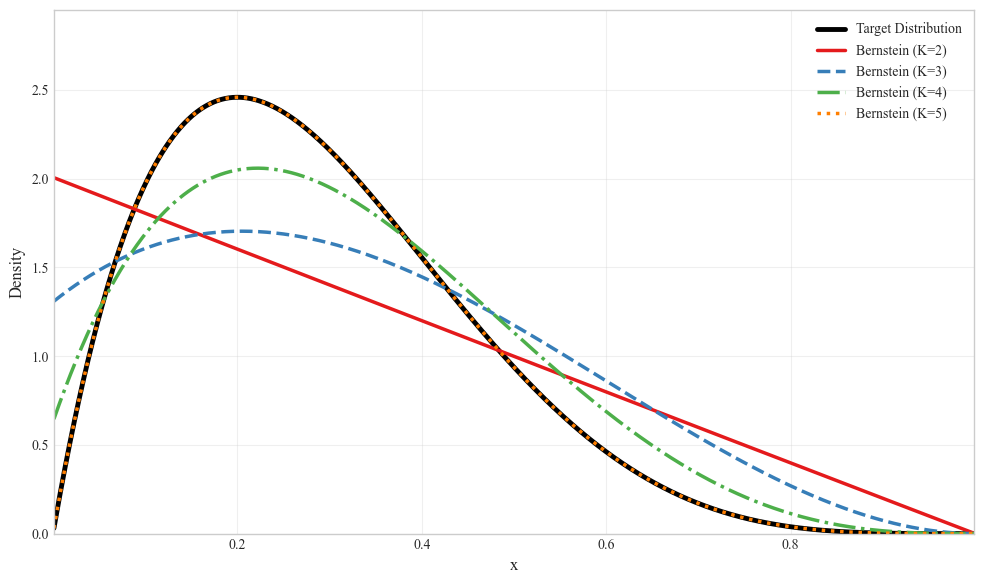
\includegraphics[width=0.5\linewidth]{figures/plot2.png}
    }
    \subfigure[$\;$ $\mbox{Kumaraswamy}(2,3)$]
    {
        \centering
        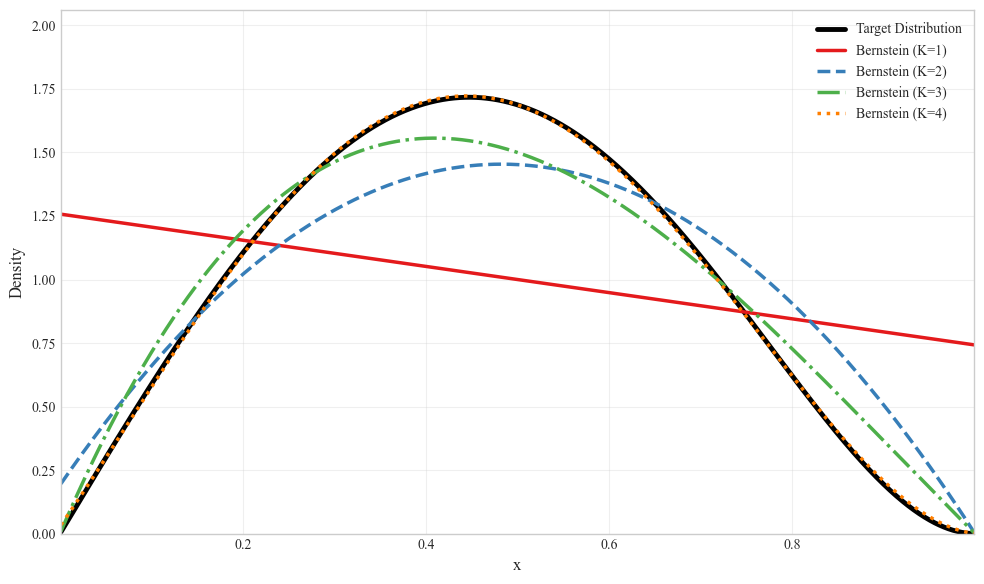
\includegraphics[width=0.5\linewidth]{figures/plot3.png}
    }
    \subfigure[$\;$ $\mbox{Triangular}(0.7)$]
    {
        \centering
        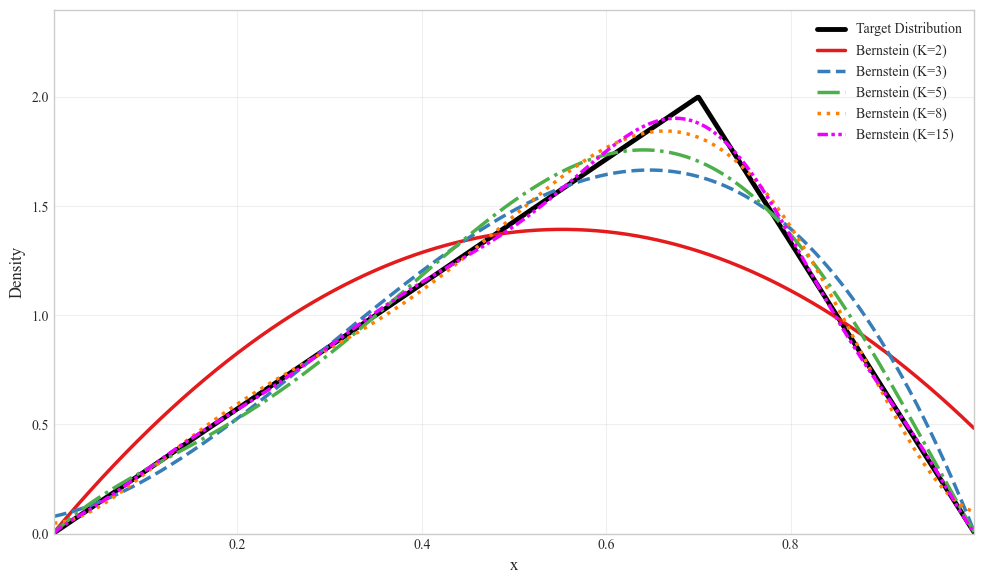
\includegraphics[width=0.5\linewidth]{figures/plot4.png}
    }
    \caption{$\;$ Bernstein approximation for various continuous distributions defined on $[0,1]$.}
\end{figure}
Figure 1 shows the approximate effect of Bernstein distribution on some common continuous distributions defined on the interval $[0,1]$. We can found that with the increase of $K$, the Bernstein distribution gradually approaches the target distribution, and finally achieves a completely approximate effect.

Based on the above theorems and conclusions, we can take Bernstein distribution as the general accurate prior distribution of the success probability $p$ in binomial distribution, which can not only expand the shape constraint prior of the original beta--binomial distribution, adapt to more complex and changeable real data, but also avoid the subjectivity and randomness of the selection of prior distribution, there is no need to preset the specific form. 